% Input data 
\subsection{Input Data}
\subsubsection{Joint states of robot}
When connection with the controller is established the joint states will be available. Each joint has a value in radians describing its state, i.e. its revolution. The objective is to build a model of the robot in camera centered coordinates where the distance to a moving object, represented as a point cloud in 3D space can be computed.
The data regarding joint states is used for both visualization, in the shape of a mesh figure, and for calculation of the robot's position in relation to other objects. These two are independent with respect to each other.

\subsubsection{Depth-image from Kinect}
The IR projector and IR camera provides a depth image of the collaboration area. The data is used for background segmentation and calibration. 

\begin{figure}[H]
\begin{center}
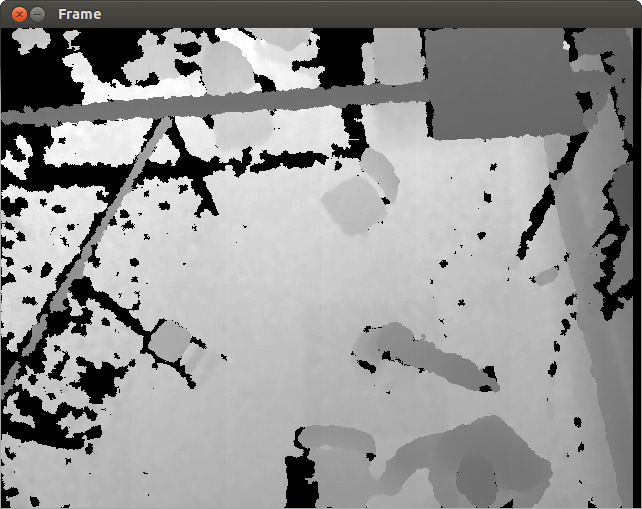
\includegraphics[width=12 cm]{screenshot_depth_image}
\caption{Depth image}

\end{center}
\end{figure}

\subsubsection{RGB-image from Kinect}
The RGB camera is used for calibration of both intrinsic and extrinsic camera parameters. From those it is possible to determine a relationship between the camera and a well known positioned calibration pattern. 

\begin{figure}[H]
\begin{center}
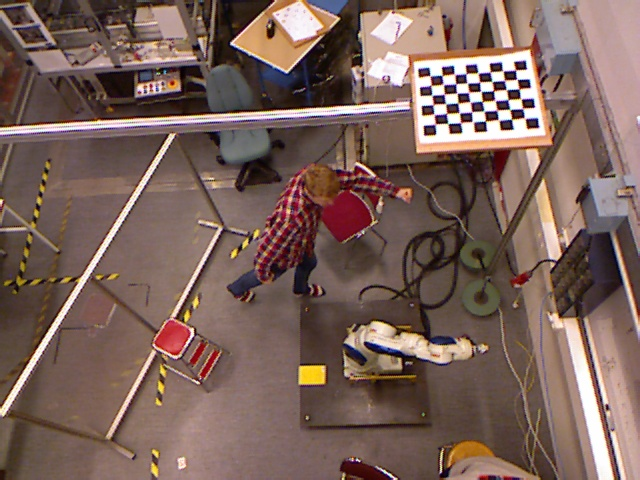
\includegraphics[width=12 cm]{image_color}
\caption{RGB-image}

\end{center}
\end{figure}
